\documentclass[11pt,a4paper]{article}
\usepackage[margin=1in]{geometry}
\usepackage{graphicx}
\usepackage{hyperref}
\usepackage{cite}
\usepackage{amsmath}
\usepackage{amssymb}
\usepackage{fancyhdr}
\usepackage{lastpage}
\usepackage{setspace}
\usepackage{booktabs}
\usepackage{float}

\pagestyle{fancy}
\fancyhf{}
\rhead{Voter ID / EPIC Assistant}
\lhead{Team Vibe Code}
\cfoot{Page \thepage\ of \pageref{LastPage}}

\setlength{\headheight}{14pt}
\onehalfspacing

\title{\textbf{Voter ID / EPIC Assistant}\\
A Retrieval-Augmented Generation (RAG) Chatbot for Government Services}

\author{
\textbf{Team: Vibe Code} \\
\\
Param Modi (2025201087) \\
Meet Ghelani (2025201096) \\
Pratee Tiwari (2025201037)
}

\date{\today}

\begin{document}

\maketitle

\begin{center}
\textbf{GitHub:} \url{https://github.com/meet6868/SMAI_ASS_3} \\[4pt]
\textbf{Live App:} \url{https://ndt6ujti6anrngsjgcdllp.streamlit.app/}
\end{center}

\begin{abstract}
This report presents a Retrieval-Augmented Generation (RAG) based chatbot designed to assist users in accessing Indian voter ID (EPIC) related services. The system retrieves relevant information from official government PDFs and generates grounded responses using large language models. It avoids model training by leveraging semantic search and external APIs. The final system is deployed as an interactive Streamlit application and supports both English and Hinglish queries.
\end{abstract}

\section{Introduction}

Accessing government services often requires users to go through multiple documents that are not easy to navigate. In the case of voter ID services, users must manually read different forms and instructions, which can be time-consuming and confusing.

To simplify this process, we developed a chatbot that allows users to ask questions in natural language. Instead of searching manually, the system retrieves relevant information from official documents and presents it in a clear and concise manner. Each answer is supported with citations, ensuring that the information is trustworthy.

\section{Data}

The system uses official voter-related forms as its data source. These include Form 6, Form 6A, Form 7, and Form 8, which cover registration, correction, and deletion processes.

The PDFs are processed through a pipeline where text is extracted, cleaned, and divided into smaller chunks. Each chunk retains metadata such as file name and page number. This metadata is later used to provide citations in the final response.

\section{Method}

\subsection{System Overview}

The system follows a Retrieval-Augmented Generation pipeline, where retrieval and generation are clearly separated. The overall workflow is shown in Figure~\ref{fig:pipeline}.

\begin{figure}[H]
\centering

\includegraphics[width=\textwidth]{/home/hp/SEM2/SMAI/Assingment/SMAI_Project/docs/diagrams/architecture_flow.png}
\caption{RAG pipeline showing document processing, embedding, retrieval, and answer generation stages.}
\label{fig:pipeline}
\end{figure}

The pipeline begins by converting PDFs into text and dividing them into overlapping chunks. These chunks are then converted into embeddings and stored in a vector database. During query time, the system retrieves the most relevant chunks and passes them to a language model, which generates the final answer.

\subsection{Embedding and Retrieval}

We use the \texttt{all-MiniLM-L6-v2} model to generate embeddings. This model is efficient and suitable for CPU-based environments. The embeddings are stored in ChromaDB, which enables fast similarity search.

At runtime:
\begin{itemize}
    \item The user query is converted into an embedding
    \item Similar chunks are retrieved using cosine similarity
    \item Top-$k$ relevant chunks are selected as context
\end{itemize}

\subsection{Answer Generation}

The retrieved chunks are passed to a language model (Gemini or Groq Llama-3). The prompt ensures that the model generates answers strictly based on the provided context. The output also includes citations pointing to the source documents.

\subsection{Query Handling}

To improve usability, the system includes a simple query expansion mechanism. For example, informal queries such as ``name change karna hai'' are expanded with voter-related context to improve retrieval accuracy.

\subsection{Key Insights}

From our experiments and usage, we observed several important behaviors of the system:

\begin{itemize}
    \item \textbf{Retrieval dominates performance:} The quality of the final answer depends heavily on the retrieved chunks. If retrieval fails, the language model produces weak or incomplete answers.
    
    \item \textbf{Chunk size trade-off:} Smaller chunks improve retrieval precision but sometimes lose context, while larger chunks preserve context but may reduce retrieval accuracy.
    
    \item \textbf{Query expansion is effective:} Simple keyword-based expansion significantly improves performance for Hinglish queries without requiring multilingual embeddings.
    
    \item \textbf{LLM variability:} Different LLM providers (Gemini vs Groq) show noticeable differences in response style and latency, even when given the same context.
    
    \item \textbf{Latency bottleneck:} Most of the response time comes from the generation step rather than retrieval.
\end{itemize}



\section{User Interface}

The system is deployed using Streamlit and provides a chat-based interface. Users can enter queries and receive responses in real time.

Key features include:
\begin{itemize}
    \item Chat interface using \texttt{st.chat\_input}
    \item Display of answers with citations
    \item Optional Hindi response mode
    \item Text-to-speech support for responses
\end{itemize}

\subsection{Interface Snapshots}

Figure~\ref{fig:ui-loading} shows the initial loading state of the deployed Streamlit app.

\begin{figure}[H]
\centering
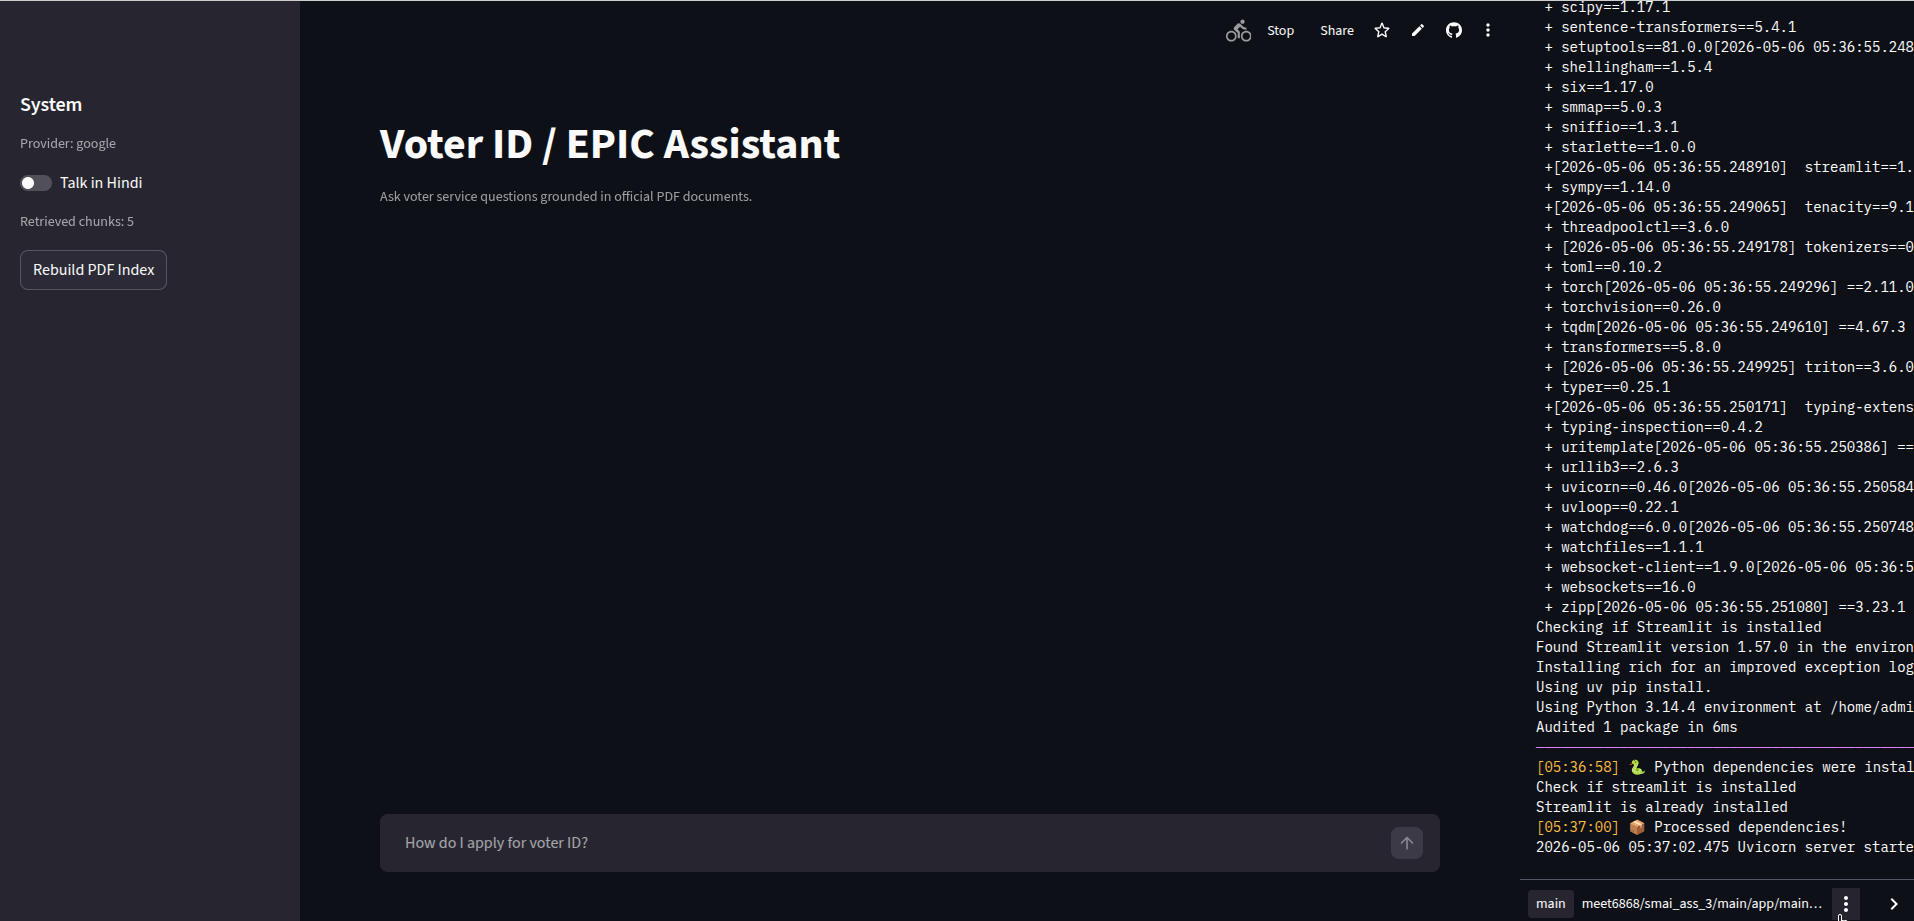
\includegraphics[width=\textwidth]{../Images/1.png}
\caption{Streamlit app loading state on deployment.}
\label{fig:ui-loading}
\end{figure}

Figure~\ref{fig:ui-english} illustrates an English query with a grounded response and citations.

\begin{figure}[H]
\centering
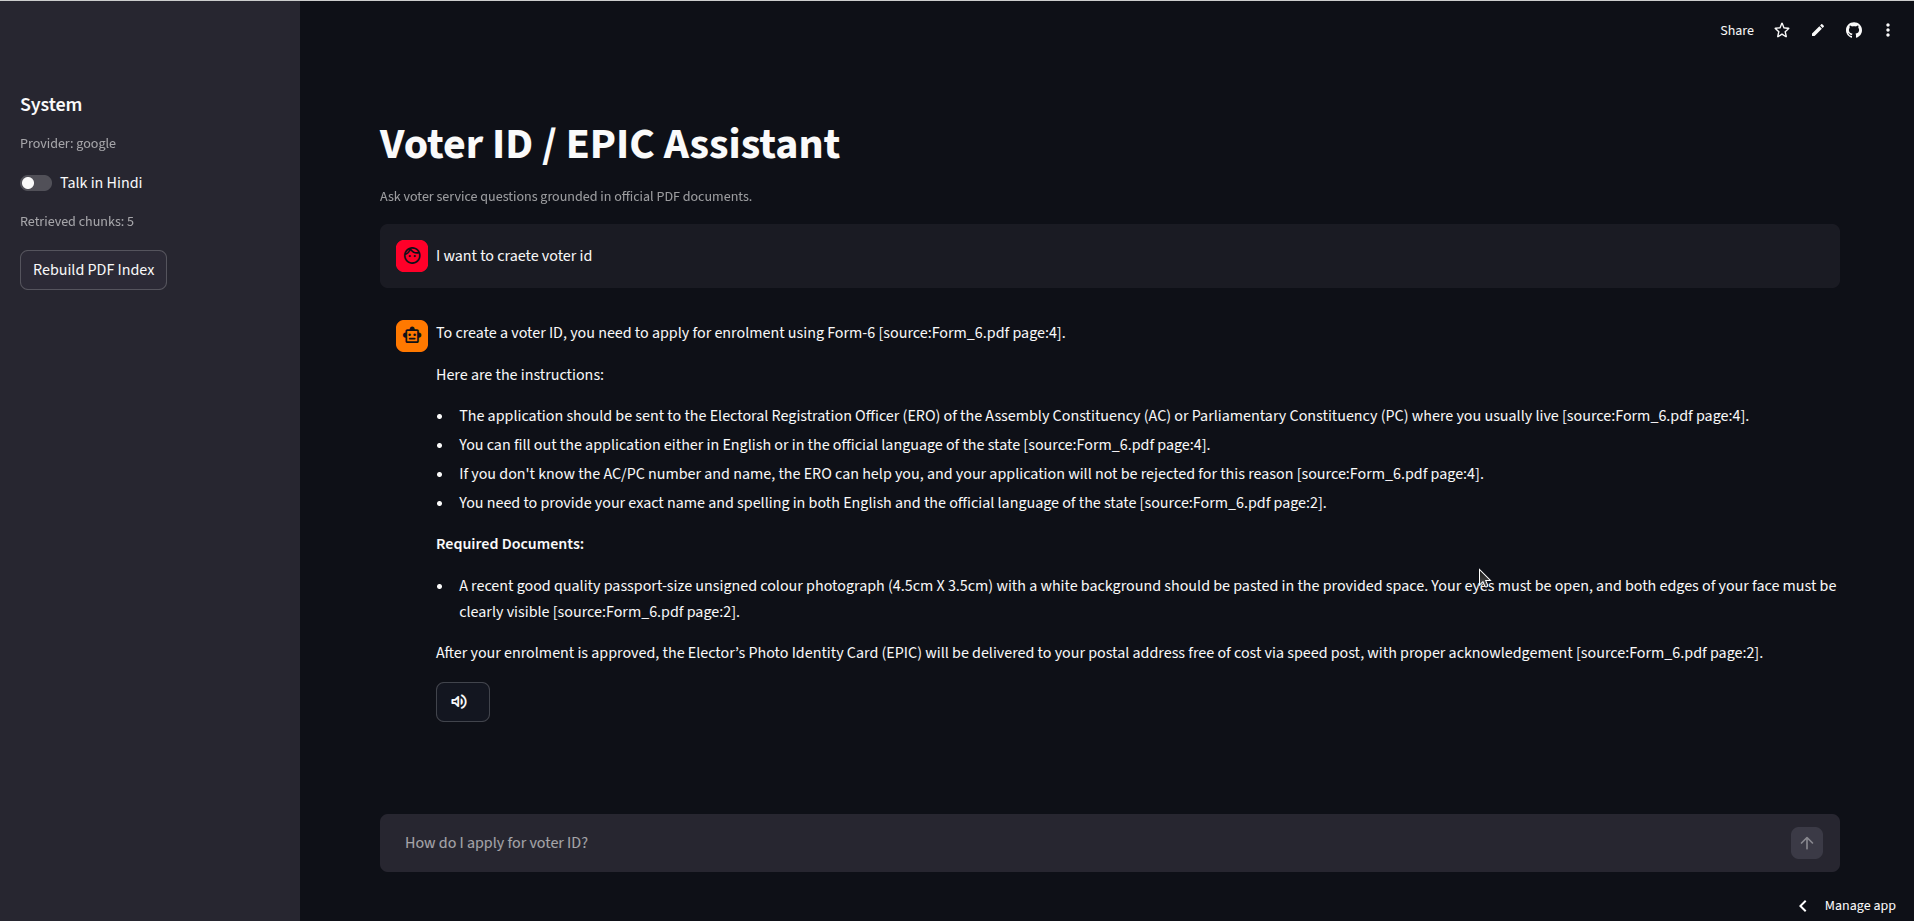
\includegraphics[width=\textwidth]{../Images/2.png}
\caption{English query and answer with sources.}
\label{fig:ui-english}
\end{figure}

Figure~\ref{fig:ui-hinglish} shows a Hinglish query where the assistant returns an English response.

\begin{figure}[H]
\centering
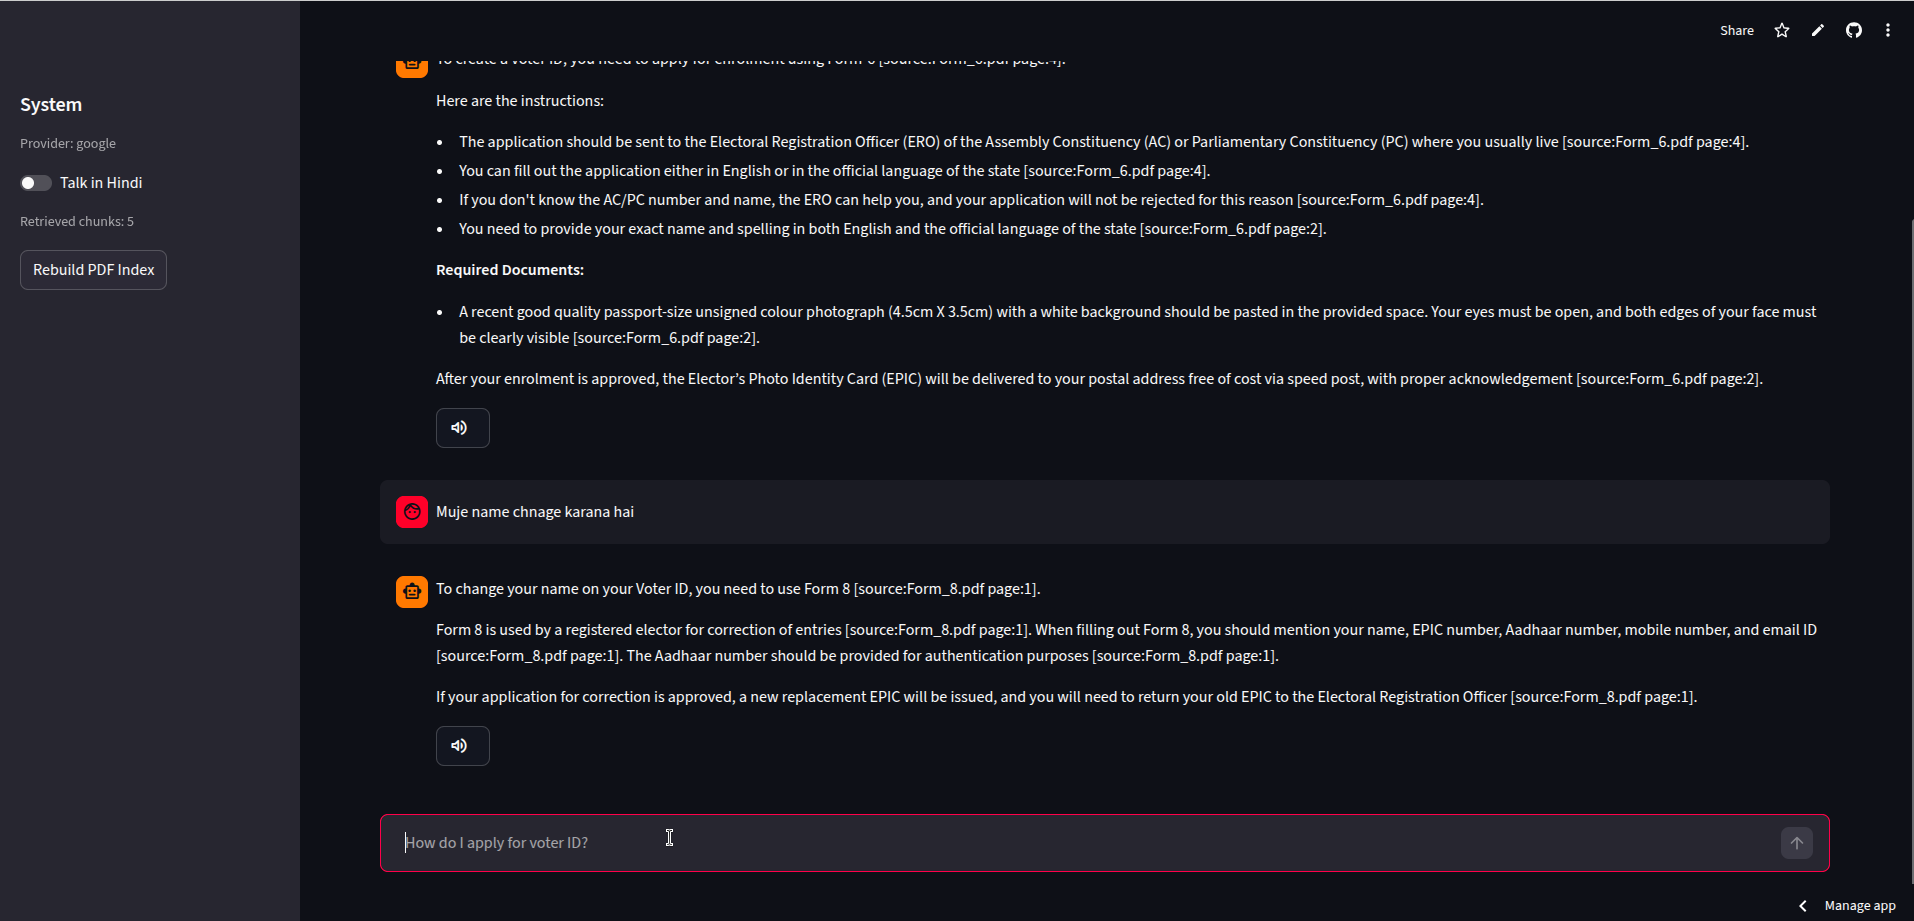
\includegraphics[width=\textwidth]{../Images/3.png}
\caption{Hinglish query with English response.}
\label{fig:ui-hinglish}
\end{figure}

Figure~\ref{fig:ui-hindi} demonstrates a Hinglish query with Hindi response mode enabled.

\begin{figure}[H]
\centering
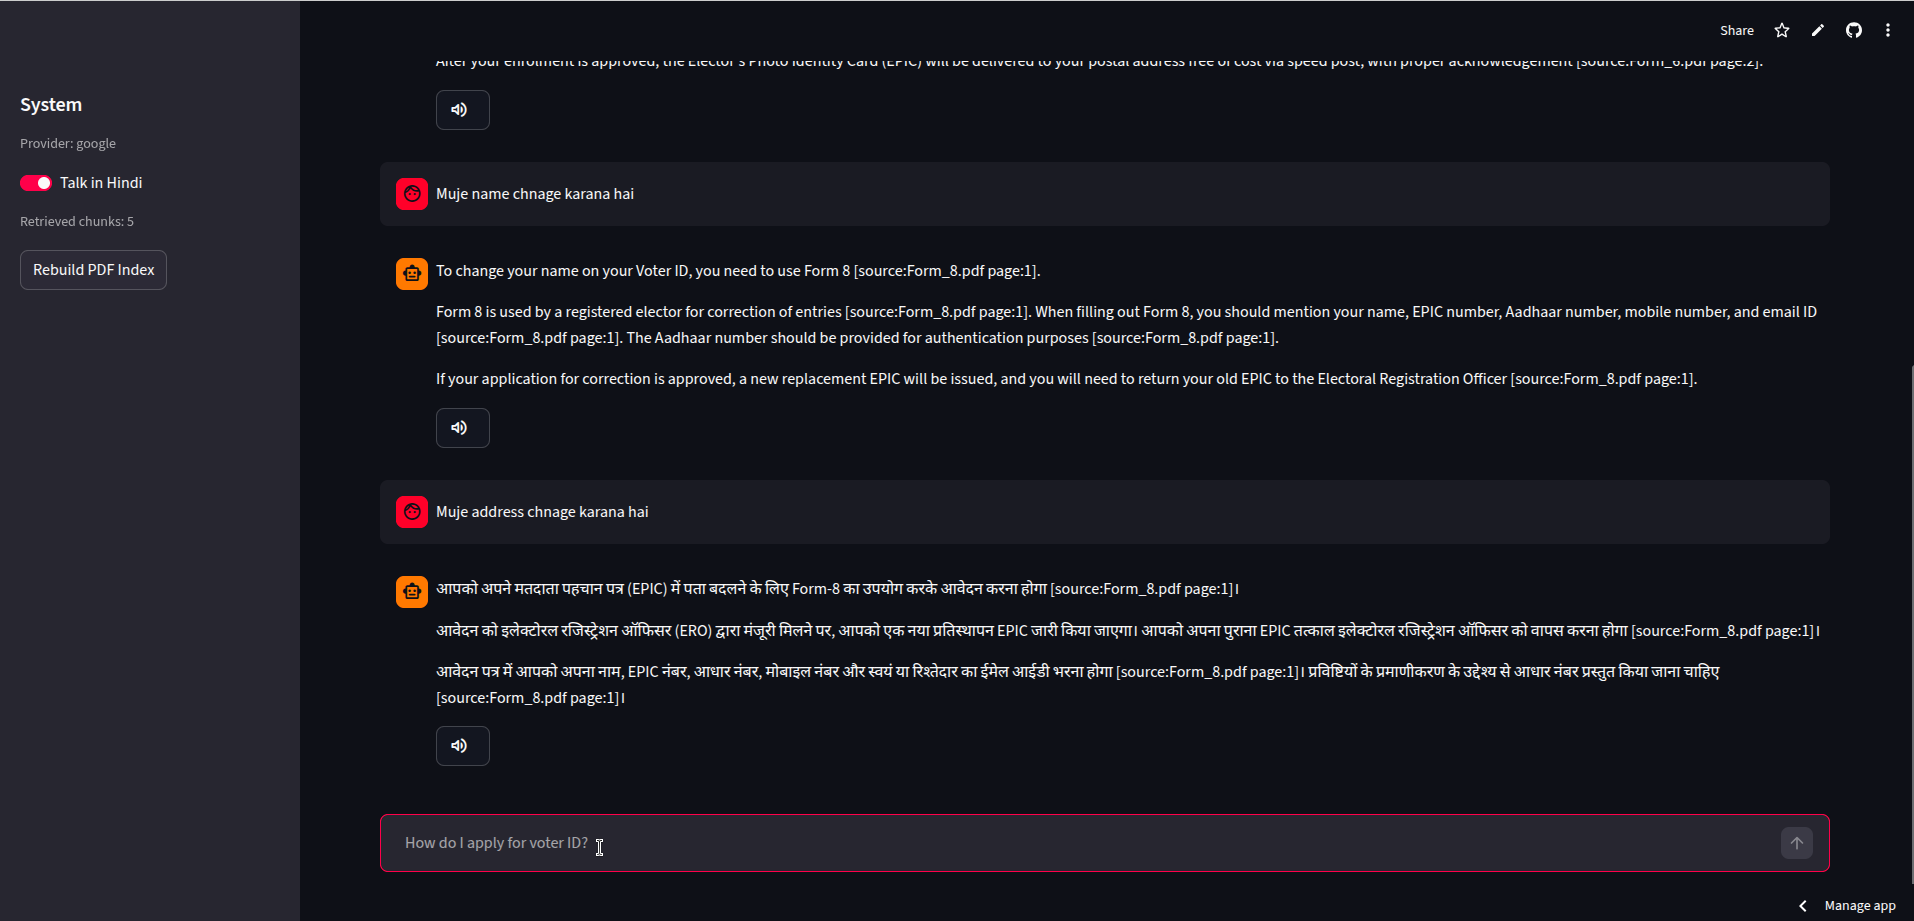
\includegraphics[width=\textwidth]{../Images/4.png}
\caption{Hinglish query with Hindi response.}
\label{fig:ui-hindi}
\end{figure}

\section{Results}

The system was evaluated using several sample queries related to voter ID services. It was observed that the chatbot retrieves relevant information and generates useful responses.

In most cases:
\begin{itemize}
    \item Retrieved documents were relevant to the query
    \item Responses were grounded in the retrieved context
    \item Citations correctly matched the source documents
\end{itemize}

The system also handled simple Hinglish queries reasonably well due to query expansion.

\subsection{Performance Measurements}

We instrumented the application to record retrieval time, generation time, end-to-end latency, and response sizes. The Streamlit app logs each query to a CSV file with prompt/answer size estimates and process memory usage. Table~\ref{tab:latency} reports the measured values from \texttt{data/metrics.csv}.

\begin{table}[H]
\centering
\scriptsize
\setlength{\tabcolsep}{3pt}
\renewcommand{\arraystretch}{1.05}
\makebox[\textwidth][c]{%
\begin{tabular}{p{5.4cm}rrrrrr}
\toprule
Query & Retrieve (ms) & Generate (ms) & End-to-end (ms) & Prompt chars & Answer chars & RSS (MB) \\
\midrule
I wanrt to create Voter Id & 26.59 & 6841.86 & 8879.71 & 4894 & 765 & 1276.04 \\
Muje name and addgress chnage karana hai & 25.10 & 6987.82 & 7012.96 & 4917 & 798 & 1277.55 \\
Muje dob chnage karani hai & 25.16 & 15174.23 & 15199.42 & 4966 & 414 & 1278.48 \\
Muje mobile no update karana hai & 25.02 & 27217.31 & 27242.38 & 4968 & 421 & 1278.80 \\
What is EPIC in voter ID? & 28.22 & 4980.10 & 5008.38 & 4892 & 381 & 1278.94 \\
How to delete my name from voter list? & 23.13 & 11578.59 & 11601.76 & 4914 & 1019 & 1279.20 \\
\bottomrule
\end{tabular}%
}
\caption{Latency and resource measurements collected from the deployed app.}
\label{tab:latency}
\end{table}


\section{Ablation Study}

Due to time and resource constraints, we did not perform a full quantitative ablation study across multiple configurations. Instead, we fixed a single pipeline setup that provided stable and reliable performance for our use case.

We selected the \texttt{all-MiniLM-L6-v2} embedding model due to its efficiency and good semantic performance in general-purpose tasks. The chunk size and overlap were chosen empirically to balance context preservation and retrieval accuracy.

We also fixed the number of retrieved chunks ($k=4$) to avoid excessive context while still providing sufficient information to the language model.

Although no systematic ablation experiments were conducted, informal testing indicated that:
\begin{itemize}
    \item Very small chunk sizes reduced context quality
    \item Very large chunks reduced retrieval precision
    \item Increasing $k$ beyond 4 did not significantly improve answers but increased latency
\end{itemize}

Future work can include controlled experiments to evaluate the impact of chunk size, retrieval depth, and different embedding models.

\section{Limitations}

Despite good performance, the system has some limitations:
\begin{itemize}
    \item Limited dataset (only a few PDF forms)
    \item Dependence on external LLM APIs
    \item Limited multilingual support
    \item Requires re-indexing when documents change
\end{itemize}

\section{Conclusion}

This project demonstrates how a RAG-based system can be used to build an effective domain-specific chatbot without training a model. By combining retrieval with language generation, the system provides accurate and explainable responses. The deployed application highlights the practical usefulness of such systems in improving access to government services.

\section*{Team Contribution}

\begin{itemize}
    \item \textbf{Param Modi (2025201087)}: Developed the core RAG pipeline
    \item \textbf{Meet Ghelani (2025201096)}: Deployment and report writing
    \item \textbf{Pratee Tiwari (2025201037)}: Streamlit UI development
\end{itemize}

\section*{Team Discussion}

All team members contributed to system design decisions, including architecture, model selection, and integration. The final system is a result of collaborative development and iterative improvements.

\section{References}

\begin{thebibliography}{99}

\bibitem{rag}
Lewis et al., Retrieval-Augmented Generation, NeurIPS 2020

\bibitem{sbert}
Reimers \& Gurevych, Sentence-BERT, EMNLP 2019

\bibitem{chromadb}
ChromaDB Documentation

\bibitem{nvsp}
\url{https://www.nvsp.in}

\bibitem{eci}
\url{https://eci.gov.in}

\end{thebibliography}

\end{document}